\documentclass[12pt,a4paper]{article}
\usepackage[utf8]{inputenc}
\usepackage[T1]{fontenc}
\usepackage[indonesian]{babel}
\usepackage{lmodern}
\usepackage{geometry}
\usepackage{amsmath,amssymb,booktabs,array,graphicx,float}
\usepackage{algorithm}
\usepackage{algpseudocode}
\usepackage{listings}
\usepackage{microtype}
\usepackage[hidelinks]{hyperref}
\geometry{margin=2.54cm}
\graphicspath{{../hasil/}{hasil/}}   % lokal: ../hasil/; Overleaf: hasil/ di samping soal1.tex
\newcommand{\R}{\mathbb{R}}
\newcommand{\T}{\mathsf{T}}
% \input biasa di dalam tabular gagal bila diikuti \bottomrule; pakai primitif \@@input
\makeatletter\newcommand{\isitabel}[1]{\@@input #1 }\makeatother

% Penomoran mengikuti nomor bagian: Tabel 2.1, Gambar 6.1, Kode 5.1, persamaan (3.1)
\numberwithin{equation}{section}
\counterwithin{table}{section}
\counterwithin{figure}{section}
\counterwithin{algorithm}{section}
\floatname{algorithm}{Kode}
\setlength{\belowcaptionskip}{6pt}   % jarak antara caption (di atas) dan tabel
\algrenewcommand\algorithmicrequire{\textbf{Masukan:}}
\algrenewcommand\algorithmicensure{\textbf{Keluaran:}}
\lstset{language=Python, basicstyle=\ttfamily\scriptsize, breaklines=true, columns=fullflexible,
  keepspaces=true, showstringspaces=false, frame=single}

\begin{document}
\begin{center}
{\Large\bfseries Soal 1: Analisis Perpindahan Penumpang Antarhalte}\par\medskip
Kelompok A12 -- TK 1 Analisis Numerik
\end{center}
\section*{Rangkuman}
Studi ini menentukan distribusi steady state untuk enam matriks perpindahan penumpang kode B, dengan 16 sampai 512 halte. Karena $I-T^\mathsf{T}$ singular, satu persamaan diganti dengan syarat skala dan solusi dinormalkan. Kami mengimplementasikan LU dense serta eliminasi pita berpivot parsial untuk matriks dengan lower bandwidth 2 dan upper bandwidth 1. Kedua solver memberi solusi dan residual yang sama pada ketelitian eksperimen. Pada $N=512$, solver pita memerlukan 60~KiB dan 20.1~ms, dibandingkan 4108~KiB dan 164.2~ms untuk dense. Kasus $N=256$ hampir terpisah menjadi dua bagian dan menghasilkan kondisi terbesar, $\kappa_1(B)\approx1.71\times10^9$. Halte terakhir memiliki proporsi maksimum pada semua ukuran. Solver pita direkomendasikan untuk koridor besar, sambil tetap memantau kondisi matriks.
\setcounter{tocdepth}{1}
\tableofcontents
\clearpage


%======================================================================
\section{Pendahuluan}
Distribusi penumpang jangka panjang pada koridor halte dapat dimodelkan sebagai distribusi stasioner rantai Markov. Tujuan studi ini ialah menghitung distribusi tersebut untuk enam matriks transisi kode B milik kelompok genap A12, dan membandingkan solver LU dense dengan solver berpivot parsial yang memanfaatkan struktur pita. Kami memeriksa validitas data, mengatasi singularitas sistem stasioner dengan satu syarat skala, lalu mengukur waktu, memori, kondisi, dan galat. Hasil dipakai untuk menentukan metode yang tepat ketika jumlah halte membesar.\par

\section{Data dan Validasi}\label{sec:data}

\subsection{Deskripsi data}
Sebuah koridor memiliki $N$ halte bernomor $1,\dots,N$ sesuai urutan lokasinya. Misalkan $X_k$ adalah halte tempat
seorang penumpang berada pada interval waktu ke-$k$. Matriks transisi $T\in\R^{N\times N}$ berisi
$T_{ij}=\Pr(X_{k+1}=j\mid X_k=i)$, yaitu peluang penumpang berpindah dari halte $i$ ke halte $j$ dalam satu interval.
Data kode B terdiri atas enam berkas \texttt{T\_N.csv} untuk $N\in\{16,32,64,128,256,512\}$, masing-masing berisi
$N$ baris dan $N$ kolom bilangan riil tanpa header. Pada keenam berkas, elemen tak-nol hanya terletak pada kolom
$j\in\{i-1,i,i+1,i+2\}$. Dalam satu interval, penumpang hanya dapat mundur satu halte, tetap, atau maju satu hingga dua
halte, sehingga setiap baris memuat dua sampai empat elemen tak-nol dan $T$ berstruktur pita (\emph{banded}).

\subsection{Prosedur validasi}
Setiap matriks dibaca dengan fungsi \texttt{baca\_T} lalu diperiksa oleh \texttt{validasi\_T}
(Lampiran~\ref{lamp:kode}). Pemeriksaan pertama menyangkut bentuk data: $T$ harus berukuran $N\times N$ sesuai nama
berkas, seluruh elemennya hingga (bukan NaN atau Inf), dan $T_{ij}\ge0$ karena setiap elemen adalah peluang.
Jumlah setiap baris harus satu. Data disimpan sebagai bilangan titik-mengambang, jadi syarat ini diperiksa dengan
toleransi, yaitu $\max_i\bigl\lvert\sum_{j=1}^{N}T_{ij}-1\bigr\rvert\le\tau$ dengan $\tau=10^{-12}$. Nilai $\tau$
jauh di atas epsilon mesin presisi ganda, $\varepsilon=2^{-53}\approx1.11\times10^{-16}$~\cite{heath}, tetapi cukup
kecil untuk mendeteksi kesalahan data.

Syarat berikutnya menjamin distribusi \emph{steady state} tunggal. Rantai Markov berhingga yang \emph{irreducible},
yaitu setiap halte dapat dicapai dari setiap halte lain, memiliki tepat satu distribusi stasioner dan seluruh
komponennya positif~\cite{norris}. Untuk memeriksanya, $T$ dipandang sebagai graf berarah $G$ dengan simpul berupa
halte dan sisi $i\to j$ jika $T_{ij}>0$. Rantai irreducible jika dan hanya jika $G$ terhubung kuat. Hal ini
diperiksa dengan dua \emph{breadth-first search} (BFS)~\cite{cormen} dari halte~1. BFS pertama dijalankan pada $G$
untuk memastikan semua halte dapat dicapai dari halte~1, dan BFS kedua pada $G$ dengan arah sisi dibalik untuk
memastikan halte~1 dapat dicapai dari semua halte. Sebagai pemeriksaan tambahan, rantai juga harus aperiodik agar
distribusi penumpang konvergen ke distribusi stasioner dari kondisi awal apa pun~\cite{norris}. Untuk rantai
irreducible, cukup ada satu $T_{ii}>0$. Karena $T$ disimpan dense, setiap BFS memindai satu baris atau kolom penuh
untuk setiap simpul, sehingga biaya validasi $O(N^2)$. Biaya ini termasuk tahap persiapan data, bukan solver.

\subsection{Hasil validasi}\label{subsec:hasilvalidasi}
\begin{table}[H]
\centering
\caption{Hasil validasi matriks transisi. Untuk semua $N$, dimensi sesuai, seluruh elemen hingga dan nonnegatif,
rantai irreducible dan aperiodik, dan setiap baris memuat 2--4 elemen tak-nol.}
\label{tab:validasi}
\begin{tabular}{rcccc}
\toprule
$N$ & $\max_i\lvert\sum_j T_{ij}-1\rvert$ & $\min_i T_{ii}$ & $\min\{T_{ij}>0: i\ne j\}$ & Valid\\
\midrule
\isitabel{generated/tabel_validasi.tex}
\bottomrule
\end{tabular}
\end{table}

Tabel~\ref{tab:validasi} menunjukkan bahwa keenam matriks lolos seluruh pemeriksaan. Galat jumlah baris maksimum
adalah $\varepsilon$ untuk $N=16$ dan $2\varepsilon=2.22\times10^{-16}$ untuk ukuran lainnya, jadi selisih tersebut
berasal dari pembulatan dan bukan dari kesalahan data. Seluruh elemen diagonal bernilai paling sedikit $0.835$,
sehingga setiap rantai aperiodik. Setiap $T$ karena itu memiliki distribusi stasioner tunggal yang positif di semua
halte. Sifat irreducible ini juga menjadi dasar bahwa matriks koefisien pada Bagian~\ref{sec:formulasi} nonsingular.
Fungsi validasi juga diuji pada empat matriks $3\times3$, yaitu satu matriks valid dan tiga matriks yang sengaja
dibuat salah (ada elemen negatif, satu baris berjumlah $0.9$, dan satu halte menyerap sehingga rantai tidak
irreducible). Keempat keputusan sesuai harapan (\texttt{hasil/uji\_validasi.csv}), jadi fungsi tersebut tidak sekadar
meloloskan semua data.

Kolom keempat Tabel~\ref{tab:validasi} memperlihatkan satu pengecualian. Pada $N=256$, peluang pindah antara halte 128
dan 129 hanya berorde $10^{-8}$, sedangkan peluang pindah positif terkecil pada matriks lain sekitar $0.014$. Total
peluang lintas dari halte 1--128 ke halte 129--256, yaitu $\sum_{i\le128<j}T_{ij}$, hanya sekitar
$9.0\times10^{-8}$, dan arah sebaliknya juga sekitar $9.0\times10^{-8}$. Matriks $T_{256}$ tetap valid karena peluang
itu positif dan rantai tetap irreducible. Namun, koridornya hampir terpecah menjadi dua blok. Dampaknya terhadap
kondisi sistem linear dibahas pada Bagian~7.

%======================================================================
\section{Formulasi dan Penanganan Singularitas}\label{sec:formulasi}
Misalkan $\pi^{(k)}\in\R^N$ adalah vektor kolom dengan $\pi^{(k)}_i=\Pr(X_k=i)$. Hukum peluang total memberi
$\pi^{(k+1)}_j=\sum_{i}\pi^{(k)}_i T_{ij}$, atau $\pi^{(k+1)}=T^\T\pi^{(k)}$. Distribusi steady state
$\pi$ adalah distribusi yang tidak berubah oleh satu langkah transisi, sehingga memenuhi
\begin{equation}\label{eq:steady}
T^\T\pi=\pi,\qquad \mathbf1^\T\pi=1,\qquad \pi_i\ge0,
\end{equation}
dengan $\mathbf1\in\R^N$ vektor yang seluruh elemennya satu. Dengan mendefinisikan $A=I-T^\T$, persamaan pertama
menjadi $A\pi=0$.

Matriks $A$ singular. Setiap baris $T$ berjumlah satu, yaitu $T\mathbf1=\mathbf1$, sehingga
\[
\mathbf1^\T A=\mathbf1^\T-(T\mathbf1)^\T=\mathbf0^\T .
\]
Jumlah seluruh baris $A$ adalah vektor nol. Baris-baris $A$ bergantung linear dan $\det A=0$, jadi eliminasi Gauss
atau faktorisasi LU tidak dapat langsung dipakai pada $A$. Hubungan yang sama menunjukkan bahwa baris pertama $A$
sama dengan $-\sum_{i\ge2}A_{i,:}$. Persamaan pertama dari $A\pi=0$ tidak membawa informasi baru~\cite{stewart}, dan
dapat diganti dengan syarat skala $z_1=1$:
\begin{equation}\label{eq:B}
B_{1,:}=e_1^\T,\qquad B_{i,:}=A_{i,:}\ (i=2,\dots,N),\qquad b=e_1,\qquad Bz=b,
\end{equation}
dengan $e_1=(1,0,\dots,0)^\T$.

Matriks $B$ nonsingular. Ekspansi kofaktor sepanjang baris pertama memberi $\det B=\det A_{2:N,2:N}$, yaitu
determinan $A$ setelah baris dan kolom halte~1 dibuang. Submatriks ini sama dengan $I-\widetilde T^\T$, dengan
$\widetilde T$ matriks transisi tanpa halte~1. Karena rantai irreducible, penumpang di halte mana pun pada akhirnya
mencapai halte~1. Peluang untuk terus berada di halte $2,\dots,N$ menuju nol, yaitu $\widetilde T^k\to0$. Akibatnya
1 bukan nilai eigen $\widetilde T$, sehingga $I-\widetilde T^\T$ dan $B$ nonsingular~\cite{stewart}.

Solusi $z$ masih perlu dinormalkan. Distribusi tunggal $\pi$ memenuhi $A_{i,:}\pi=0$ untuk $i\ge2$ dan $\pi_1>0$,
jadi solusi tunggal $Bz=b$ adalah $z=\pi/\pi_1$. Baris pertama hanya memilih skala $z_1=1$, sehingga umumnya
$\mathbf1^\T z\ne1$. Normalisasi
\begin{equation}\label{eq:normal}
\pi=\frac{z}{\mathbf1^\T z}
\end{equation}
mengembalikan syarat $\mathbf1^\T\pi=1$. Syarat $\pi_i\ge0$ ikut terpenuhi karena $z=\pi/\pi_1>0$.

%======================================================================
\section{Identifikasi Struktur Banded}\label{sec:band}
Untuk matriks $M\in\R^{N\times N}$, \emph{lower bandwidth} $p$ dan \emph{upper bandwidth} $q$ adalah
\begin{equation}\label{eq:pq}
p=\max\{\,i-j : M_{ij}\ne0\,\},\qquad q=\max\{\,j-i : M_{ij}\ne0\,\},
\end{equation}
dengan nilai $0$ jika himpunannya kosong. Matriks pita hanya memiliki elemen tak-nol pada $p$ diagonal di bawah dan
$q$ diagonal di atas diagonal utama. Fungsi \texttt{deteksi\_bandwidth} menghitung~\eqref{eq:pq} secara otomatis dari
posisi elemen tak-nol. Untuk keenam ukuran diperoleh $p=2$ dan $q=1$, baik untuk $A$ maupun $B$. Jadi $B$
\emph{bukan} tridiagonal.

Struktur ini dapat diturunkan langsung. Untuk $i\ge2$, $B_{ij}=\delta_{ij}-T_{ji}$ dengan $\delta_{ij}$ delta
Kronecker, sehingga elemen tak-nol $T$ pada posisi $j-i=d$ muncul di $B$ pada posisi $j-i=-d$. Karena posisi tak-nol
$T$ adalah $d\in\{-1,0,1,2\}$, baris $i\ge2$ dari $B$ hanya memuat
\begin{equation}\label{eq:bandB}
B_{i,i-2}=-T_{i-2,i},\quad B_{i,i-1}=-T_{i-1,i},\quad B_{ii}=1-T_{ii},\quad B_{i,i+1}=-T_{i+1,i}.
\end{equation}
Penggantian baris pertama dengan $e_1^\T$ tetap mempertahankan struktur pita. Vektor $e_1^\T$ hanya tak-nol pada
diagonal, jadi penggantian itu dapat menghapus elemen tak-nol tetapi tidak pernah menambah elemen di luar pita.

Matriks dense membutuhkan $N^2$ bilangan, sedangkan pita $B$ hanya $(p+q+1)N$. Solver dengan \emph{partial pivoting}
membutuhkan sedikit ruang tambahan. Pertukaran baris $k$ dengan baris $r\le k+p$ membawa elemen tak-nol sampai kolom
$r+q\le k+p+q$, sehingga upper bandwidth faktor $U$ dapat naik dari $q$ menjadi $p+q$ (\emph{fill-in}), sementara
lower bandwidth $L$ tetap $p$~\cite{golub}. Kami menyimpan $B$ dalam array $AB\in\R^{(2p+q+1)\times N}$ dengan format
penyimpanan pita LAPACK~\cite{lapack}: $B_{ij}$ berada di $AB_{\,p+q+1+i-j,\;j}$, sehingga setiap diagonal $B$ menjadi
satu baris $AB$ dan $p$ baris teratas dicadangkan untuk fill-in. Untuk $p=2$ dan $q=1$, array ini berukuran
$6\times N$.

\begin{table}[H]
\centering
\caption{Kebutuhan memori penyimpanan $B$ dalam byte (\texttt{float64}, 8 byte per elemen): dense $N^2$,
pita $(p+q+1)N$, dan pita dengan ruang fill-in $(2p+q+1)N$. Rasio = dense dibagi pita dengan fill-in.}
\label{tab:storage}
\begin{tabular}{rrrrr}
\toprule
$N$ & Dense & Pita & Pita + fill-in & Rasio\\
\midrule
\isitabel{generated/tabel_storage.tex}
\bottomrule
\end{tabular}
\end{table}

Tabel~\ref{tab:storage} menunjukkan bahwa rasio penyimpanan dense terhadap pita dengan ruang fill-in sama dengan
$N/6$. Keunggulan penyimpanan pita tumbuh linear terhadap $N$. Pada $N=512$, matriks dense membutuhkan 2 MiB,
sedangkan pita hanya 24 KiB, atau sekitar 85 kali lebih kecil.

%======================================================================
\section{Metode Penyelesaian}\label{sec:metode}
Kedua solver diimplementasikan sendiri dalam \texttt{soal1/soal1.ipynb}. NumPy hanya dipakai untuk array,
\emph{indexing}, dan aritmetika dasar; tidak ada pustaka penyelesaian SPL atau faktorisasi di dalam solver.
Fungsi \texttt{np.linalg.solve} hanya dipakai pada sel verifikasi yang diberi label terpisah. Matriks permutasi $P$
disimpan sebagai vektor indeks.

\subsection{LU dense dengan partial pivoting}
Solver (a) menghitung $PB=LU$ dengan $L$ segitiga bawah berdiagonal satu, $U$ segitiga atas, dan $P$ matriks
permutasi~\cite{heath}. Pada langkah $k$, baris dengan $\lvert B_{ik}\rvert$ terbesar ($i\ge k$) ditukar ke posisi
$k$. Pertukaran dilakukan pada seluruh baris, termasuk multiplier yang sudah tersimpan, agar $L$ konsisten dengan $P$
akhir. Multiplier $\ell_{ik}=B_{ik}/B_{kk}$ disimpan di tempat elemen yang dieliminasi, sehingga $L$ dan $U$ berbagi
satu array $N\times N$. Sistem kemudian diselesaikan dengan substitusi maju $Ly=Pb$ dan substitusi mundur $Uz=y$.
Langkah-langkah ini dirangkum pada Kode~\ref{alg:dense} dan diimplementasikan pada fungsi \texttt{lu\_dense} dan
\texttt{solve\_lu}.

\begin{algorithm}[H]
\caption{LU dense dengan \emph{partial pivoting} dan penyelesaian $Bz=b$}
\label{alg:dense}
\begin{algorithmic}[1]
\Require $B\in\R^{N\times N}$ nonsingular, $b\in\R^N$
\Ensure $z\in\R^N$ dengan $Bz=b$
\State $M\gets B$ (salinan); $\mathit{perm}\gets(1,2,\dots,N)$
\For{$k=1$ \textbf{to} $N-1$}
  \State $r\gets\arg\max_{k\le i\le N}\lvert M_{ik}\rvert$; \textbf{if} $M_{rk}=0$ \textbf{then error} ``singular''
  \State Tukar baris $M_{k,:}\leftrightarrow M_{r,:}$ dan $\mathit{perm}_k\leftrightarrow\mathit{perm}_r$
  \Comment{seluruh baris}
  \For{$i=k+1$ \textbf{to} $N$}
    \State $M_{ik}\gets M_{ik}/M_{kk}$ \Comment{multiplier $\ell_{ik}$}
    \State $M_{i,k+1:N}\gets M_{i,k+1:N}-M_{ik}\,M_{k,k+1:N}$
  \EndFor
\EndFor
\State $y\gets b_{\mathit{perm}}$ \Comment{$y=Pb$}
\For{$i=2$ \textbf{to} $N$} \Comment{substitusi maju $Ly=Pb$}
  \State $y_i\gets y_i-\sum_{j<i}M_{ij}y_j$
\EndFor
\For{$i=N$ \textbf{downto} $1$} \Comment{substitusi mundur $Uz=y$}
  \State $z_i\gets\bigl(y_i-\sum_{j>i}M_{ij}z_j\bigr)/M_{ii}$
\EndFor
\State \Return $z$
\end{algorithmic}
\end{algorithm}

\subsection{Solver banded bergaya Thomas}
Solver (b) harus berjalan dalam $O(N)$ waktu dan memori. Algoritma Thomas klasik memenuhi syarat ini, tetapi hanya
berlaku untuk matriks tridiagonal ($p=q=1$), sedangkan $B$ memiliki $p=2$ dan $q=1$. Solver (b) karena itu berupa
perluasannya untuk matriks pita umum, yaitu eliminasi Gauss dengan partial pivoting yang hanya bekerja di dalam
pita~\cite{golub}, langsung pada array $AB$ dari Bagian~\ref{sec:band}. Algoritmanya ada pada Kode~\ref{alg:band} (fungsi \texttt{bentuk\_B\_band},
\texttt{lu\_band}, dan \texttt{solve\_band}).

Ada tiga hal yang membuat solver ini berjalan dalam $O(N)$. Pertama, pita diambil langsung dari $T$: fungsi
\texttt{bentuk\_B\_band} mengisi $AB$ menurut~\eqref{eq:bandB} dan hanya mengakses $N(p+q+1)$ elemen $T$, jadi
matriks $B$ dense, $L$, $U$, maupun $P$ berukuran $N\times N$ tidak pernah dibentuk. Kedua, pivot hanya dicari di
baris $k,\dots,\min(N,k+p)$ karena di bawahnya kolom $k$ sudah nol, sedangkan pertukaran dan pembaruan hanya
menyentuh kolom $k,\dots,\min(N,k+p+q)$. Ketiga, multiplier langkah sebelumnya tidak ikut ditukar seperti pada
Kode~\ref{alg:dense}, karena tersimpan di kolom lain $AB$. Indeks pertukaran setiap langkah dicatat di vektor
$\mathit{piv}$, lalu diulang dengan urutan yang sama pada ruas kanan saat substitusi maju. Hasilnya setara dengan
$PB=LU$.

\begin{algorithm}[H]
\caption{Faktorisasi dan penyelesaian banded dengan \emph{partial pivoting}. Notasi $B_{ij}$ berarti elemen yang
disimpan di $AB_{p+q+1+i-j,\,j}$.}
\label{alg:band}
\begin{algorithmic}[1]
\Require $AB\in\R^{(2p+q+1)\times N}$ berisi pita $B$, $p$, $q$, $b\in\R^N$
\Ensure $z\in\R^N$ dengan $Bz=b$
\For{$k=1$ \textbf{to} $N$}
  \State $i_{\max}\gets\min(N,k+p)$; \quad $j_{\max}\gets\min(N,k+p+q)$
  \State $r\gets\arg\max_{k\le i\le i_{\max}}\lvert B_{ik}\rvert$; \textbf{if} $B_{rk}=0$ \textbf{then error}
  ``singular''
  \State $\mathit{piv}_k\gets r$; tukar $B_{kj}\leftrightarrow B_{rj}$ untuk $j=k,\dots,j_{\max}$
  \For{$i=k+1$ \textbf{to} $i_{\max}$}
    \State $B_{ik}\gets B_{ik}/B_{kk}$ \Comment{multiplier $\ell_{ik}$}
    \State $B_{ij}\gets B_{ij}-B_{ik}B_{kj}$ untuk $j=k+1,\dots,j_{\max}$
  \EndFor
\EndFor
\State $y\gets b$
\For{$k=1$ \textbf{to} $N$} \Comment{maju: ulangi pertukaran dan eliminasi}
  \State tukar $y_k\leftrightarrow y_{\mathit{piv}_k}$; \quad
         $y_i\gets y_i-B_{ik}y_k$ untuk $i=k+1,\dots,\min(N,k+p)$
\EndFor
\For{$i=N$ \textbf{downto} $1$} \Comment{mundur: $U$ selebar $p+q$}
  \State $z_i\gets\bigl(y_i-\sum_{j=i+1}^{\min(N,i+p+q)}B_{ij}z_j\bigr)/B_{ii}$
\EndFor
\State \Return $z$
\end{algorithmic}
\end{algorithm}

\subsection{Uji kebenaran}
Sebelum dipakai pada data, kedua solver diuji pada matriks kecil yang hasilnya dapat dicek manual
(Tabel~\ref{tab:uji}). Pada uji~2, hitungan tangan dengan dua kali pertukaran baris memberi
\[
L=\begin{pmatrix}1&0&0\\0.25&1&0\\0.5&2/3&1\end{pmatrix},\qquad
U=\begin{pmatrix}8&7&9\\0&-0.75&-1.25\\0&0&-2/3\end{pmatrix},\qquad
\mathit{perm}=(3,1,2),
\]
dengan $\mathit{perm}$ urutan baris $B$ setelah permutasi $P$. Kedua solver menghasilkan faktor yang sama persis.

\begin{table}[H]
\centering
\caption{Uji kebenaran pada matriks kecil.}
\label{tab:uji}
\small
\begin{tabular}{@{}>{\raggedright}p{0.34\textwidth}>{\raggedright}p{0.12\textwidth}>{\raggedright\arraybackslash}p{0.44\textwidth}@{}}
\toprule
Kasus & Solver & Hasil\\
\midrule
1. Matriks valid dan tiga matriks rusak $3\times3$ (Bagian~\ref{sec:data}) & validasi & keempat keputusan sesuai\\
2. $B=\left(\begin{smallmatrix}2&1&1\\4&3&3\\8&7&9\end{smallmatrix}\right)$, $b=(3,7,19)^\T$
   & dense, banded ($p=q=2$) & $L$, $U$, $P$ sama dengan hitungan tangan; $\max\lvert PB-LU\rvert=0$;
   $z=(1,-1,2)^\T$\\
3. Matriks $4\times4$ dengan $B_{11}=0$ & dense & baris 1 dan 2 ditukar; galat solusi $4.4\times10^{-16}$\\
4. Matriks pita $8\times8$, $p=2$, $q=1$, diagonal diperkecil 100 kali & banded vs dense & 7 pertukaran baris,
   8 elemen fill-in, $U$ melebar tepat sampai $p+q=3$; $P$ dan $U$ identik dengan solver dense;
   galat solusi $5.3\times10^{-15}$\\
5. Matriks singular $\left(\begin{smallmatrix}1&2\\2&4\end{smallmatrix}\right)$ & dense, banded &
   keduanya menolak karena pivot nol\\
6. Rantai \emph{birth--death} $3\times3$ dengan $\pi=(\tfrac14,\tfrac12,\tfrac14)^\T$ & dense, banded &
   $\pi$ tepat sama\\
\bottomrule
\end{tabular}
\end{table}

Pada keenam data, pivoting tidak pernah menukar baris (\texttt{hasil/akurasi\_dense.csv} dan
\texttt{hasil/akurasi\_band.csv}). Penyebabnya, $B$ dominan diagonal per kolom. Pada kolom $k\ge2$ berlaku
$\lvert B_{kk}\rvert=1-T_{kk}=\sum_{i\ne k}T_{ki}\ge\sum_{i\ne k,\,i\ge2}\lvert B_{ik}\rvert$, dan pada kolom pertama
$B_{11}=1\ge T_{12}+T_{13}$. Eliminasi Gauss mempertahankan sifat ini, sehingga partial pivoting selalu memilih elemen
diagonal~\cite{golub}. Jalur pertukaran baris karena itu hanya teruji lewat uji~2--4 pada Tabel~\ref{tab:uji}.

Tanpa pertukaran baris, kedua solver melakukan operasi titik-mengambang yang sama pada angka yang sama; solver dense
hanya menambah operasi terhadap elemen nol. Hasilnya, $\pi$ dari solver banded identik dengan $\pi$ dari solver dense,
dengan selisih maksimum $0$ pada mesin kami, karena tanpa pertukaran baris kedua solver melakukan operasi yang sama. Sebagai pembanding independen, selisih terhadap
\texttt{np.linalg.solve} paling besar $2.6\times10^{-16}$ untuk $N\ne256$ dan $6.6\times10^{-13}$ untuk $N=256$
(\texttt{hasil/verifikasi\_*\_numpy.csv}). Selisih yang lebih besar pada $N=256$ sejalan dengan struktur yang hampir
terpecah pada Subbagian~\ref{subsec:hasilvalidasi} dan dianalisis pada Bagian~7.

%======================================================================
\section{Eksperimen Kinerja dan Analisis Kompleksitas}\label{sec:eksperimen}

\subsection{Rancangan eksperimen}
Eksperimen dijalankan pada AMD Ryzen 7 7435HS dengan RAM 16 GB, Windows 11, Python 3.14.4, dan NumPy 2.5.3.
Waktu solver adalah waktu faktorisasi, substitusi, dan normalisasi~\eqref{eq:normal}. Waktu membaca CSV dan
persiapan diukur terpisah. Persiapan solver dense adalah pembentukan $B$ dense, yang berbiaya $O(N^2)$. Persiapan
solver banded adalah deteksi $p$ dan $q$ dari posisi tak-nol $T$, yang juga $O(N^2)$ karena data masukan dense,
ditambah ekstraksi pita yang $O(N)$. Waktu diukur dengan \texttt{time.perf\_counter}. Setelah satu kali pemanasan,
setiap pengukuran diulang 15 kali dan diambil nilai minimumnya, karena gangguan dari sistem operasi hanya dapat
menambah waktu. Memori diukur dengan dua cara: puncak alokasi selama solver berjalan menurut \texttt{tracemalloc},
dan total \texttt{.nbytes} array yang disimpan solver (koefisien, ruas kanan, faktor, vektor pivot, dan solusi).
Seluruh hasil tersimpan di \texttt{hasil/benchmark.csv}.

\subsection{Hasil}
\begin{table}[H]
\centering
\caption{Waktu (ms, minimum dari 15 ulangan) dan memori (KiB) untuk data soal.}
\label{tab:bench}
\small
\setlength{\tabcolsep}{4pt}
\begin{tabular}{r rrrrr rrrr}
\toprule
 & Baca & \multicolumn{2}{c}{Dense (ms)} & \multicolumn{2}{c}{Banded (ms)} & \multicolumn{2}{c}{\texttt{.nbytes}} &
 \multicolumn{2}{c}{Peak}\\
\cmidrule(lr){3-4}\cmidrule(lr){5-6}\cmidrule(lr){7-8}\cmidrule(lr){9-10}
$N$ & CSV & persiapan & solver & persiapan & solver & dense & banded & dense & banded\\
\midrule
\isitabel{generated/tabel_benchmark.tex}
\bottomrule
\end{tabular}
\end{table}

\begin{figure}[H]
\centering
\includegraphics[width=0.78\textwidth]{waktu_vs_N.png}
\caption{Waktu solver terhadap $N$ (skala log--log). Marker kosong dan garis putus-putus adalah rantai sintetis
$N=1024$ dan $2048$; garis abu-abu adalah garis bantu $\propto N^3$ dan $\propto N$.}
\label{fig:waktu}
\end{figure}

Tabel~\ref{tab:bench} dan Gambar~\ref{fig:waktu} menunjukkan bahwa keunggulan solver banded baru muncul pada $N$
sedang. Untuk $N\le64$, solver banded 1.5--1.8 kali lebih lambat daripada solver dense, dan pada $N=128$ keduanya
setara. Setiap langkah solver banded berupa perulangan Python kecil dengan biaya tetap, sedangkan setiap langkah
solver dense adalah satu operasi vektor NumPy yang dieksekusi dalam kode terkompilasi. Pada $N$ kecil, waktu lebih
ditentukan oleh banyaknya langkah daripada banyaknya flop. Mulai $N=256$ solver banded lebih cepat, yaitu 1.9 kali
pada $N=256$ dan 8.2 kali pada $N=512$. Pada $N=512$, waktu membaca CSV (29.4~ms) bahkan sudah melebihi waktu solver
banded (20.1~ms). Untuk melihat tren pada $N$ yang lebih besar, kedua solver juga dijalankan pada rantai sintetis
$N=1024$ dan $2048$ dengan pola pita yang sama (bukan data soal, lima ulangan). Pada $N=2048$, solver dense
membutuhkan 12.7~s, sedangkan solver banded hanya 83~ms.

\begin{figure}[H]
\centering
\includegraphics[width=0.78\textwidth]{memori_vs_N.png}
\caption{Memori terhadap $N$. Garis tebal menunjukkan total \texttt{.nbytes} array yang disimpan solver; garis
bertitik dengan marker silang menunjukkan puncak \texttt{tracemalloc}.}
\label{fig:memori}
\end{figure}

Perbedaan memori pada Gambar~\ref{fig:memori} lebih tegas daripada perbedaan waktu. Total \texttt{.nbytes} solver
dense naik empat kali setiap $N$ digandakan, sedangkan solver banded hanya naik dua kali. Pada $N=512$, solver dense
menyimpan 4108~KiB dan solver banded 60~KiB, sekitar 68 kali lebih kecil. Puncak \texttt{tracemalloc} mengikuti pola
yang sama.

\subsection{Analisis kompleksitas}
Banyaknya operasi dihitung dalam flop: satu flop adalah satu pasangan perkalian dan pengurangan, atau satu
pembagian. Pada solver dense, langkah $k$ mengeliminasi $N-k$ baris dan tiap baris memperbarui $N-k$ elemen,
sehingga faktorisasi memerlukan $\sum_{k=1}^{N-1}(N-k)^2\approx N^3/3$ flop~\cite{heath}. Substitusi maju dan
mundur masing-masing sekitar $N^2/2$ flop. Array faktornya berukuran $N^2$. Jadi solver dense membutuhkan $O(N^3)$
waktu dan $O(N^2)$ memori.

Pada solver banded, setiap kolom hanya mengeliminasi $p$ baris, dan setiap baris hanya memperbarui $p+q$ elemen
karena faktor $U$ melebar akibat pivoting. Faktorisasi memerlukan sekitar
\begin{equation}\label{eq:flopband}
N\,p\,(p+q)
\end{equation}
flop, yaitu $6N$ untuk $p=2$ dan $q=1$; taksiran $(p+q)^2N/4$ yang lebih kecil berlaku untuk eliminasi pita tanpa
pivoting. Substitusi maju dan mundur hanya menyentuh elemen di dalam pita, sehingga biayanya $O(N(p+q))$. Memori yang
dibutuhkan adalah array $AB$ berukuran $(2p+q+1)N$. Untuk $p$ dan $q$ tetap, waktu dan memori sama-sama $O(N)$,
sesuai yang dituntut dari solver (b). Sebagai gambaran, pada $N=512$ faktorisasi dense memerlukan sekitar
$4.5\times10^{7}$ flop, sedangkan faktorisasi banded hanya 3072 flop (\texttt{hasil/flop\_teori.csv}).

\begin{table}[H]
\centering
\caption{Kemiringan garis log--log (pangkat empiris $N$) terhadap nilai teoretis. Kolom terakhir memakai
$N=256$, $512$ dan dua titik sintetis.}
\label{tab:slope}
\begin{tabular}{lcccc}
\toprule
Besaran & Teori & $N=16$--$512$ & $N=128$--$512$ & $N=256$--$2048$\\
\midrule
\isitabel{generated/tabel_kemiringan.tex}
\bottomrule
\end{tabular}
\end{table}

Tabel~\ref{tab:slope} membandingkan teori dengan eksperimen melalui kemiringan garis terbaik pada skala log--log,
yang dihitung dengan rumus regresi linear sederhana. Kemiringan waktu solver banded sekitar 1 pada semua rentang,
sesuai $O(N)$. Kemiringan waktu solver dense hanya 1.71 pada seluruh data karena pada $N$ kecil biaya tetap setiap
langkah masih dominan, lalu naik menjadi 2.56 untuk $N\ge128$ dan 3.18 untuk $N\ge256$, mendekati $N^3$. Kemiringan flop
faktorisasi dan \texttt{.nbytes} sama dengan teori: 3 dan 2 untuk dense, 1 untuk banded. Eksperimen ini mengonfirmasi analisis di
atas: solver banded linear dalam waktu dan memori, sedangkan solver dense kuadratik dalam memori dan mendekati kubik
dalam waktu.

%======================================================================
\section{Analisis Kondisi dan Galat}\label{sec:kondisi}

\subsection{Ukuran yang dihitung}
Bagian ini menimbang tiga hal: kondisi $B$ sebagai sifat masalah, galat residual sebagai sifat algoritma, dan galat
maju sebagai akibat dari keduanya. Kondisi $B$ diukur dengan bilangan kondisi norma-1
\begin{equation}\label{eq:kappa}
\kappa_1(B)=\lVert B\rVert_1\,\lVert B^{-1}\rVert_1,\qquad
\lVert M\rVert_1=\max_{j}\sum_{i}\lvert M_{ij}\rvert,
\end{equation}
yang dipakai untuk seluruh $N$ agar nilainya dapat dibandingkan antarukuran. Norma-1 dipilih karena nilainya
diperoleh eksak dari jumlah mutlak kolom, sedangkan norma-2 memerlukan nilai singular yang tidak dapat dihitung tanpa
pustaka faktorisasi~\cite{heath}. Matriks $B^{-1}$ dibentuk dengan menyelesaikan $BX=I$ memakai faktor $PB=LU$ dari
solver dense, yaitu substitusi maju dan mundur untuk semua kolom sekaligus (Kode~\ref{alg:kappa}; fungsi
\texttt{invers\_dari\_LU} dan \texttt{bilangan\_kondisi\_1}). Biayanya $O(N^3)$, yang masih dapat diterima untuk
$N\le2048$. Untuk $N$ yang jauh lebih besar, $\kappa_1$ cukup ditaksir dengan estimator Hager--Higham, yang hanya
memerlukan penyelesaian sistem dengan $B$ dan $B^\T$ memakai faktor yang sudah ada~\cite{higham}. Fungsi ini diuji
pada matriks $3\times3$ dari Tabel~\ref{tab:uji} (uji~2): invers sama dengan hitungan tangan dan
$\kappa_1=14\times5.5=77$.

\begin{algorithm}[H]
\caption{Bilangan kondisi $\kappa_1(B)$ dari faktor $PB=LU$}
\label{alg:kappa}
\begin{algorithmic}[1]
\Require $B\in\R^{N\times N}$, faktor $L,U$ dan vektor permutasi $\mathit{perm}$ dari Kode~\ref{alg:dense}
\Ensure $\kappa_1(B)$
\State $Y\gets I_{\mathit{perm},:}$ \Comment{$Y=PI$}
\For{$i=2$ \textbf{to} $N$} \Comment{substitusi maju untuk semua kolom: $LY=PI$}
  \State $Y_{i,:}\gets Y_{i,:}-\sum_{j<i}L_{ij}\,Y_{j,:}$
\EndFor
\For{$i=N$ \textbf{downto} $1$} \Comment{substitusi mundur: $UX=Y$, sehingga $X=B^{-1}$}
  \State $X_{i,:}\gets\bigl(Y_{i,:}-\sum_{j>i}U_{ij}\,X_{j,:}\bigr)/U_{ii}$
\EndFor
\State \Return $\bigl(\max_j\sum_i\lvert B_{ij}\rvert\bigr)\bigl(\max_j\sum_i\lvert X_{ij}\rvert\bigr)$
\end{algorithmic}
\end{algorithm}

Selain $r=\lVert T^\T\hat\pi-\hat\pi\rVert_2$ dan $e_{\mathrm{norm}}=\lvert\mathbf1^\T\hat\pi-1\rvert$ yang diminta
soal, kami menghitung dua ukuran tambahan. Yang pertama adalah galat mundur relatif
\begin{equation}\label{eq:eta}
\eta=\frac{\lVert b-B\hat z\rVert_1}{\lVert B\rVert_1\,\lVert\hat z\rVert_1},
\end{equation}
yaitu seberapa kecil gangguan relatif pada $B$ yang membuat $\hat z$ menjadi solusi eksak~\cite{higham}. Yang kedua
adalah galat maju $\delta=\lVert\hat\pi-\pi^\ast\rVert_1$ terhadap solusi acuan $\pi^\ast$. Karena
$\lVert\pi^\ast\rVert_1=1$, $\delta$ adalah galat relatif norma-1. Acuan harus lebih akurat daripada presisi ganda.
Membandingkan kedua solver satu sama lain tidak membantu karena hasilnya identik (Subbagian~\ref{subsec:analisiskondisi}),
dan \texttt{np.linalg.solve} juga berasal dari eliminasi dengan pembulatan. Karena itu $\pi^\ast$ dihitung dengan
perbaikan iteratif dengan residual eksak (Kode~\ref{alg:acuan}). $\hat z$ diubah menjadi bilangan rasional, residual
$b-B\zeta$ dihitung eksak dengan modul \texttt{fractions} Python (hanya di dalam pita), koreksi dihitung dengan faktor
$LU$ yang sama, dan langkah ini diulang empat kali. Setiap iterasi memperkecil galat kira-kira dengan faktor
$\kappa_1\varepsilon$~\cite{higham}. Pada kasus terburuk ($\kappa_1\varepsilon\approx1.9\times10^{-7}$) galat acuan
setelah empat iterasi karena itu jauh di bawah $\delta$ yang diukur.

\begin{algorithm}[H]
\caption{Solusi acuan $\pi^\ast$ dan galat maju $\delta$ dengan perbaikan iteratif dan residual eksak}
\label{alg:acuan}
\begin{algorithmic}[1]
\Require $B$ (pita $p,q$), $b$, faktor $LU$ dan $\mathit{perm}$, solusi $\hat z$ dan $\hat\pi$, jumlah iterasi $K=4$
\Ensure $\delta=\lVert\hat\pi-\pi^\ast\rVert_1$
\State $\zeta\gets\hat z$ sebagai bilangan rasional (tepat)
\For{$k=1$ \textbf{to} $K$}
  \State $\rho\gets b-B\zeta$ \Comment{aritmetika rasional, hanya elemen di dalam pita}
  \State $d\gets$ solusi $LUd=P\rho$ dengan $\rho$ dibulatkan ke presisi ganda \Comment{substitusi Kode~\ref{alg:dense}}
  \State $\zeta\gets\zeta+d$ \Comment{penjumlahan eksak}
\EndFor
\State $\pi^\ast\gets\zeta/\mathbf1^\T\zeta$ \Comment{eksak}
\State \Return $\sum_i\lvert\hat\pi_i-\pi^\ast_i\rvert$ \Comment{dihitung eksak, lalu dibulatkan}
\end{algorithmic}
\end{algorithm}

Ketiga ukuran dihubungkan oleh pertidaksamaan sederhana. Karena $\hat z-z=B^{-1}(B\hat z-b)$,
\begin{equation}\label{eq:galatmaju}
\frac{\lVert\hat z-z\rVert_1}{\lVert\hat z\rVert_1}
\le\lVert B^{-1}\rVert_1\frac{\lVert b-B\hat z\rVert_1}{\lVert\hat z\rVert_1}
=\kappa_1(B)\,\eta .
\end{equation}
Galat maju dengan demikian dibatasi oleh hasil kali sifat masalah ($\kappa_1$) dan sifat algoritma ($\eta$). Eliminasi
Gauss yang stabil mundur memberi $\eta$ sekitar $\varepsilon=2^{-53}$~\cite{higham}, sehingga $\kappa_1\varepsilon$
lazim dipakai sebagai tolok ukur galat maju. Kami melaporkan keduanya. Residual pada~\eqref{eq:eta} dihitung dalam presisi
ganda, jadi nilainya hanya dapat dibaca sampai orde $\varepsilon$ dan~\eqref{eq:galatmaju} dipakai sebagai petunjuk orde,
bukan batas yang pasti.

\subsection{Hubungan $\kappa_1(B)$ dengan waktu pencapaian halte~1}
Untuk matriks $B$ ini, $\kappa_1(B)$ memiliki tafsiran fisik yang eksak. Misalkan $m_j$ adalah rata-rata banyaknya
interval waktu yang diperlukan penumpang dari halte $j$ untuk pertama kali tiba di halte~1 (\emph{hitting time}).

\medskip\noindent\textbf{Proposisi.}
$\kappa_1(B)=\lVert B\rVert_1\,\max\bigl\{1/\pi_1,\ \max_{j\ge2}m_j\bigr\}$.

\smallskip\noindent\emph{Bukti.}
Semua elemen $B^{-1}$ nonnegatif (ditunjukkan di bawah), sehingga $\lVert B^{-1}\rVert_1$ adalah jumlah kolom terbesar.
Kolom pertama adalah $B^{-1}e_1=z=\pi/\pi_1$ (Bagian~\ref{sec:formulasi}), yang berjumlah $1/\pi_1$. Untuk $j\ge2$, kolom
$x=B^{-1}e_j$ memenuhi $x_1=0$ (baris pertama $B$), dan komponen sisanya memenuhi
$(I-\widetilde T^\T)x_{2:N}=e_j$ dengan $\widetilde T$ seperti pada Bagian~\ref{sec:formulasi}. Karena $\widetilde T^k\to0$,
$x_{2:N}=\sum_{k\ge0}(\widetilde T^\T)^ke_j\ge0$. Komponen ke-$i$ adalah rata-rata banyaknya kunjungan ke halte $i$
sebelum penumpang yang berangkat dari halte $j$ tiba di halte~1, sehingga jumlah komponennya adalah $m_j$~\cite{norris}.
\hfill$\square$

\medskip
Proposisi ini menyatakan bahwa buruknya kondisi $B$ sama dengan lamanya penumpang dari halte terjauh mencapai halte~1.
Dua akibatnya menjelaskan Tabel~\ref{tab:kondisi}.

Pertama, rantai pada koridor ini berdifusi. Peluang pindah di bagian dalam koridor adalah sekitar $0.09$ (mundur satu
halte), $0.06$ (maju satu), dan $0.015$ (maju dua), sehingga variansi perpindahan per interval adalah
$\sigma^2=0.09+0.06+4(0.015)\approx0.21$ dengan kecenderungan arah (\emph{drift}) hampir nol
(Subbagian~\ref{subsec:mekanisme}). Untuk langkah acak seperti ini, waktu pencapaian dari ujung jauh koridor
berorde $N^2/\sigma^2$~\cite{norris}, sehingga $\kappa_1(B)=O(N^2)$. Hal ini sesuai dengan Tabel~\ref{tab:kondisi}:
$\kappa_1$ naik 3.9--4.0 kali setiap $N$ digandakan dari 16 sampai 128, dan $\kappa_1/N^2$ hampir konstan (6.2--6.6 pada data). Pada rantai
sintetis dengan drift nol, $\kappa_1/N^2=5.11$--$5.12$, sama dengan $\lVert B\rVert_1/\sigma^2=1.075/0.21$, dengan $\lVert B\rVert_1=1.075$ dari kolom pertama
($1+0.06+0.015$). Nilai pada data sedikit lebih besar. Penyebab yang mungkin adalah peluang mundur di dekat halte~1 pada
data yang lebih kecil daripada $0.09$ (misalnya $T_{21}=0.0651$), sehingga penumpang lebih lama mencapai halte~1.

Kedua, pada $N=256$ penumpang di halte 129--256 hanya dapat mencapai halte~1 dengan melintasi sambungan yang peluangnya
sekitar $9\times10^{-8}$ per interval (Subbagian~\ref{subsec:hasilvalidasi}). Aliran rata-rata melintas dari blok kedua
adalah $\pi_{129}T_{129,128}\approx3.8\times10^{-3}\cdot9.0\times10^{-8}\approx3.4\times10^{-10}$ per interval, sedangkan
blok itu menampung kira-kira separuh massa $\pi$. Waktu keluar rata-rata dari blok kedua karena itu berorde $10^{9}$
interval, sesuai dengan $\kappa_1(B)\approx1.7\times10^{9}$ karena $\lVert B\rVert_1$ berorde satu. Perhitungan ini
hanya taksiran orde besar, tetapi menunjukkan bahwa lonjakan $\kappa_1$ pada $N=256$ berasal dari struktur data, bukan dari
algoritma.

\subsection{Hasil}\label{subsec:hasilkondisi}
Seluruh nilai dihitung untuk kedua solver. Residual, $\eta$, $e_{\mathrm{norm}}$, dan $\delta$ identik pada keduanya
sampai semua angka yang disimpan (\texttt{hasil/kondisi\_galat.csv}), sehingga tabel hanya memuat satu kolom untuk
tiap besaran. Baris $N=1024$ dan $2048$ adalah rantai sintetis dari Bagian~\ref{sec:eksperimen}.

\begin{table}[H]
\centering
\caption{Kondisi dan galat residual ($\kappa_1$ pada norma-1, $r$ pada norma-2, $\eta$ pada norma-1). Nilai sama untuk
solver dense dan banded. Dua baris terakhir adalah rantai sintetis.}
\label{tab:kondisi}
\small
\setlength{\tabcolsep}{5pt}
\begin{tabular}{rcccccc}
\toprule
$N$ & $\kappa_1(B)$ & $\kappa_1/N^2$ & $r$ & $r/\lVert\hat\pi\rVert_2$ & $\eta$ & $e_{\mathrm{norm}}$\\
\midrule
16 & $1.68\times10^{3}$ & $6.55$ & $1.55\times10^{-17}$ & $6.07\times10^{-17}$ & $1.31\times10^{-17}$ & $0$ \\
32 & $6.52\times10^{3}$ & $6.36$ & $1.30\times10^{-17}$ & $7.21\times10^{-17}$ & $1.06\times10^{-17}$ & $0$ \\
64 & $2.57\times10^{4}$ & $6.27$ & $9.66\times10^{-18}$ & $7.60\times10^{-17}$ & $1.09\times10^{-17}$ & $0$ \\
128 & $1.02\times10^{5}$ & $6.23$ & $5.95\times10^{-18}$ & $6.62\times10^{-17}$ & $1.29\times10^{-17}$ & $0$ \\
256 & $1.71\times10^{9}$ & $2.61\times10^{4}$ & $3.85\times10^{-18}$ & $6.07\times10^{-17}$ & $9.88\times10^{-18}$ & $0$ \\
512 & $1.62\times10^{6}$ & $6.19$ & $3.21\times10^{-18}$ & $7.15\times10^{-17}$ & $1.11\times10^{-17}$ & $0$ \\
\midrule
1024 & $5.36\times10^{6}$ & $5.11$ & $4.19\times10^{-17}$ & $1.34\times10^{-15}$ & $1.02\times10^{-17}$ & $0$ \\
2048 & $2.15\times10^{7}$ & $5.12$ & $4.17\times10^{-17}$ & $1.89\times10^{-15}$ & $1.12\times10^{-17}$ & $0$ \\
\bottomrule
\end{tabular}
\end{table}

\begin{table}[H]
\centering
\caption{Galat maju terhadap solusi acuan eksak ($\delta$ pada norma-1) dan pembandingnya. Nilai $\delta$ sama untuk
solver dense dan banded, dan $\max_i\lvert\hat\pi^{\mathrm{dense}}_i-\hat\pi^{\mathrm{band}}_i\rvert=0$ pada semua $N$.
$\varepsilon=2^{-53}$.}
\label{tab:galatmaju}
\small
\begin{tabular}{rcccc}
\toprule
$N$ & $\kappa_1\eta$ & $\kappa_1\varepsilon$ & $\delta$ & $\delta/(\kappa_1\varepsilon)$\\
\midrule
16 & $2.20\times10^{-14}$ & $1.86\times10^{-13}$ & $4.24\times10^{-16}$ & $2.28\times10^{-3}$ \\
32 & $6.92\times10^{-14}$ & $7.24\times10^{-13}$ & $8.02\times10^{-16}$ & $1.11\times10^{-3}$ \\
64 & $2.80\times10^{-13}$ & $2.85\times10^{-12}$ & $1.09\times10^{-14}$ & $3.81\times10^{-3}$ \\
128 & $1.32\times10^{-12}$ & $1.13\times10^{-11}$ & $1.57\times10^{-14}$ & $1.39\times10^{-3}$ \\
256 & $1.69\times10^{-8}$ & $1.90\times10^{-7}$ & $5.75\times10^{-11}$ & $3.03\times10^{-4}$ \\
512 & $1.79\times10^{-11}$ & $1.80\times10^{-10}$ & $8.64\times10^{-14}$ & $4.79\times10^{-4}$ \\
\midrule
1024 & $5.49\times10^{-11}$ & $5.95\times10^{-10}$ & $4.65\times10^{-13}$ & $7.82\times10^{-4}$ \\
2048 & $2.40\times10^{-10}$ & $2.38\times10^{-9}$ & $2.03\times10^{-13}$ & $8.50\times10^{-5}$ \\
\bottomrule
\end{tabular}
\end{table}

\begin{figure}[H]
\centering
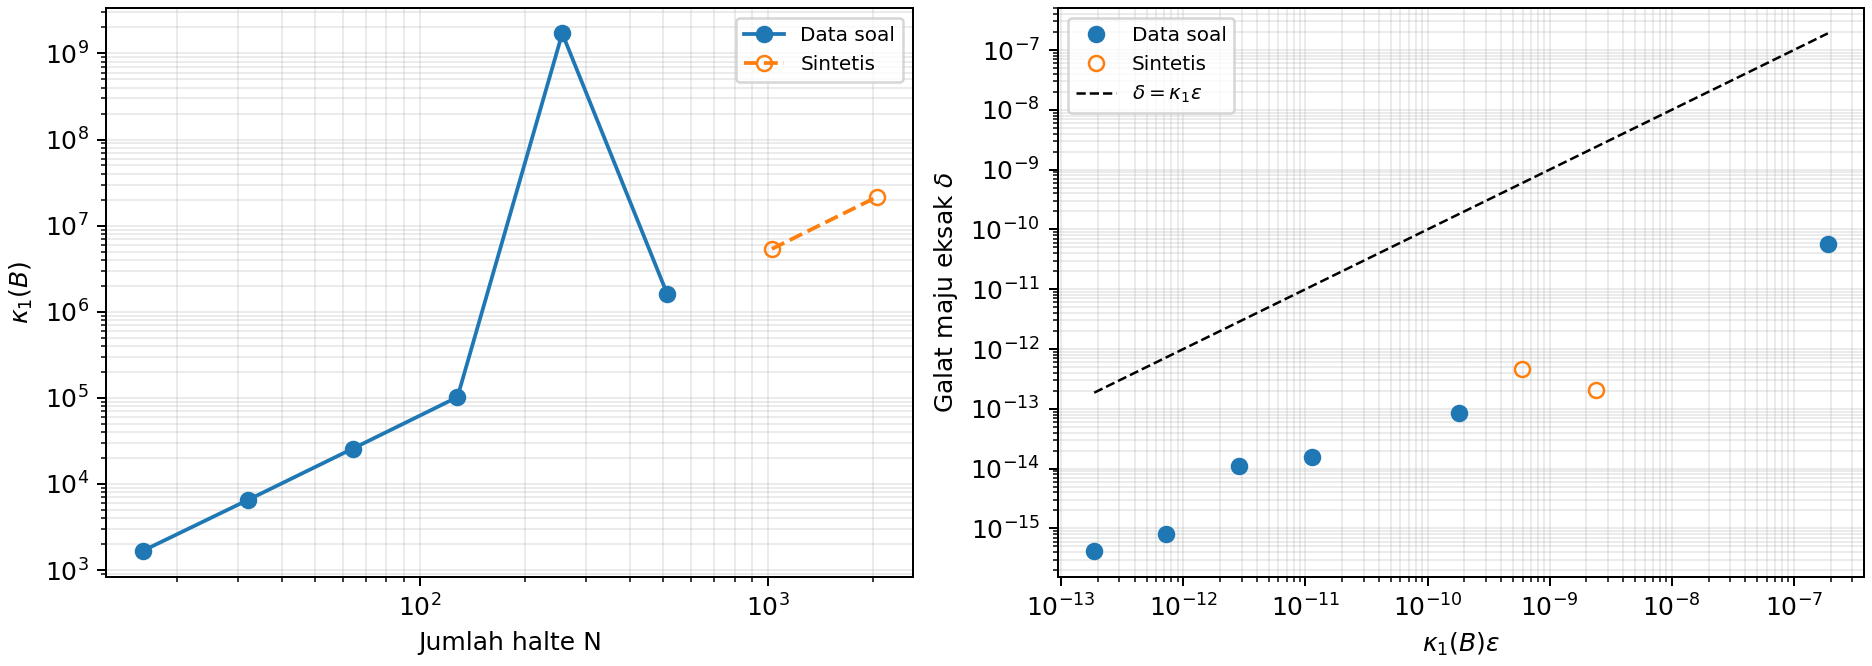
\includegraphics[width=\textwidth]{kondisi_vs_N.png}
\caption{Kiri: $\kappa_1(B)$ terhadap $N$ (skala log--log); garis putus-putus dan marker kosong adalah rantai sintetis.
Kanan: galat maju eksak $\delta$ terhadap indikator $\kappa_1\varepsilon$; semua titik berada di bawah garis
$\delta=\kappa_1\varepsilon$.}
\label{fig:kondisi}
\end{figure}

\subsection{Analisis}\label{subsec:analisiskondisi}
Tabel~\ref{tab:kondisi} dan~\ref{tab:galatmaju} menunjukkan empat pola.

Pertama, residual tidak mengikuti $\kappa_1$. Residual $r$ berada pada orde $10^{-18}$--$10^{-17}$ dan $\eta$ pada orde
$10^{-17}$ untuk semua $N$, padahal $\kappa_1(B)$ merentang dari $1.68\times10^{3}$ sampai $1.71\times10^{9}$. Pada
data, $r/\lVert\hat\pi\rVert_2$ berada di $6.1$--$7.6\times10^{-17}$, kira-kira $0.5$--$0.7\,\varepsilon$, jadi residual
sudah sekecil yang dapat dicapai presisi ganda. Hal ini sesuai dengan sifat algoritma: $B$ dominan diagonal per kolom,
sehingga eliminasi Gauss tidak memerlukan pertukaran baris dan faktor pertumbuhan elemennya paling besar 2~\cite{higham},
jadi stabil mundur. Pada rantai sintetis $r/\lVert\hat\pi\rVert_2$ sekitar $10^{-15}$, lebih besar tetapi tetap kecil;
penyebabnya tidak kami telusuri.

Kedua, galat maju mengikuti $\kappa_1$ sebagai batas atas. Nilai $\delta$ naik dari $4.24\times10^{-16}$ ($N=16$,
$\kappa_1=1.68\times10^{3}$) menjadi $5.75\times10^{-11}$ ($N=256$, $\kappa_1=1.71\times10^{9}$). Pada seluruh baris
$\delta<\kappa_1\eta$ dan $\delta/(\kappa_1\varepsilon)$ berada di antara $8.5\times10^{-5}$ dan $3.8\times10^{-3}$,
sehingga~\eqref{eq:galatmaju} berlaku tetapi konservatif sekitar dua sampai empat orde besaran. Hubungannya batas atas,
bukan prediksi: $\delta$ pada $N=2048$ ($2.03\times10^{-13}$) lebih kecil daripada pada $N=1024$ ($4.65\times10^{-13}$)
walaupun $\kappa_1$-nya lebih besar. Residual yang kecil juga tidak menjamin galat maju yang kecil. Pada $N=256$,
$r=3.85\times10^{-18}$ lebih kecil daripada pada $N=16$ ($1.55\times10^{-17}$), tetapi $\delta$ sekitar
$1.4\times10^{5}$ kali lebih besar. Sebaliknya $e_{\mathrm{norm}}=0$ pada semua $N$ dan kedua solver. Ini bukan bukti
akurasi: normalisasi~\eqref{eq:normal} memaksa $\mathbf1^\T\hat\pi=1$, jadi $e_{\mathrm{norm}}$ hanya memeriksa langkah
normalisasi dan tidak menilai ketepatan komponen $\hat\pi_i$.

Ketiga, $N=256$ adalah kasus kondisi buruk. Dari $N=128$ ke $256$, $\kappa_1$ naik $1.7\times10^{4}$ kali dan $\delta$ naik
$3.7\times10^{3}$ kali. Selisih terhadap \texttt{np.linalg.solve} pada $N=256$ ($6.6\times10^{-13}$, Bagian~\ref{sec:metode})
juga jauh lebih besar daripada ukuran lain ($\le2.6\times10^{-16}$). Selisih itu sama ordenya dengan galat per komponen,
$\delta/N\approx2.2\times10^{-13}$. Dua eliminasi yang sama-sama benar tetapi berbeda urutan pembulatannya berselisih
sebesar yang diizinkan kondisi masalah. Kondisi buruk tidak berarti hasilnya cacat: $\hat\pi$ tetap mulus di sambungan
($\pi_{129}/\pi_{128}=0.9986$) dan masih benar sampai sekitar sepuluh digit. Artinya $\hat\pi$ sensitif terhadap gangguan
pada $T$ dan pembulatan~\cite{chomeyer}. Berdasarkan Proposisi, $\kappa_1$ kira-kira berbanding terbalik dengan peluang
sambungan; bila sambungan makin lemah dan $\kappa_1\varepsilon$ mendekati satu, tidak ada digit yang dijamin benar.

Keempat, solver dense dan banded tidak dapat dibedakan. Selisih $\hat\pi$ keduanya nol pada semua $N$, dan $r$, $\eta$,
$e_{\mathrm{norm}}$, serta $\delta$ juga sama persis. Penyebabnya tidak ada pertukaran baris pada data
(Bagian~\ref{sec:metode}), sehingga kedua solver mengeksekusi pembagian dan pengurangan yang sama pada elemen tak-nol
yang sama; solver dense hanya menambah operasi dengan nol, yang tidak mengubah hasil. Kesamaan persis ini berlaku pada
mesin kami. Pada mesin atau pustaka lain, urutan penjumlahan pada substitusi dapat berbeda dan selisih berorde
$\varepsilon$ mungkin muncul, jauh di bawah $\delta$. Kesimpulannya, galat solusi ditentukan oleh kondisi masalah dan
algoritma eliminasi yang sama-sama dipakai kedua solver, bukan oleh cara penyimpanan matriks. Solver banded menghemat
waktu dan memori tanpa mengorbankan akurasi.

%======================================================================
\section{Interpretasi Hasil}\label{sec:interpretasi}

\subsection{Prosedur}
Distribusi yang dianalisis adalah $\hat\pi$ dari solver banded, yang identik dengan hasil solver dense
(Bagian~\ref{sec:kondisi}). Pada semua $N$, $\hat\pi_i>0$ untuk setiap $i$ dan $\mathbf1^\T\hat\pi=1$ (diperiksa dengan
\texttt{assert} di notebook), sesuai teori untuk rantai irreducible~\cite{norris}. Karena jumlah halte berbeda-beda,
proporsi dibandingkan dengan distribusi seragam $1/N$ lewat $N\hat\pi_i$; nilai 1 berarti halte menampung penumpang
sebanyak rata-rata. Kode~\ref{alg:interpretasi} merangkum perhitungan yang dipakai: halte dengan proporsi terbesar,
halte yang berada dalam 1\% dari maksimum, waktu kembali rata-rata $m_i=1/\pi_i$~\cite{norris}, drift per halte
$\mu_i=\sum_j(j-i)T_{ij}$, pemeriksaan keseimbangan arus, dan ekstrapolasi Richardson. Ekstrapolasi dipakai karena
nilai $N\hat\pi_{i^\ast}$ konvergen dengan galat $O(1/N)$ (Subbagian~\ref{subsec:hasilinterpretasi}), sehingga
$v_\infty\approx2v(2N)-v(N)$ menghilangkan suku galat utamanya.

\begin{algorithm}[H]
\caption{Ringkasan dan diagnosis distribusi steady state}
\label{alg:interpretasi}
\begin{algorithmic}[1]
\Require $T$ dan $\hat\pi$ untuk setiap $N\in\{16,32,\dots,512\}$
\Ensure $i^\ast$, himpunan $\mathcal H$, $m_{i^\ast}$, drift $\mu$, galat keseimbangan, $v_\infty$
\State $i^\ast\gets\arg\max_i\hat\pi_i$; \quad $i_\ast\gets\arg\min_i\hat\pi_i$
\State $\mathcal H\gets\{\,i:\hat\pi_i\ge0.99\,\hat\pi_{i^\ast}\}$ \Comment{halte dalam 1\% dari maksimum}
\State $m_{i^\ast}\gets1/\hat\pi_{i^\ast}$ \Comment{waktu kembali rata-rata ke halte terpadat}
\State $\mu_i\gets\sum_j(j-i)T_{ij}$ untuk semua $i$
\State $g\gets\max_i\bigl\lvert\hat\pi_i(1-T_{ii})-\sum_{j\ne i}\hat\pi_jT_{ji}\bigr\rvert$ \Comment{keseimbangan arus; harus mendekati 0}
\State $v(N)\gets N\hat\pi_{i^\ast}$; \quad $v_\infty\gets2v(2N)-v(N)$ \Comment{ekstrapolasi Richardson}
\State \Return $i^\ast$, $\mathcal H$, $m_{i^\ast}$, $\mu$, $g$, $v_\infty$
\end{algorithmic}
\end{algorithm}

\subsection{Hasil}\label{subsec:hasilinterpretasi}
Gambar~\ref{fig:pi} memuat $\hat\pi_i$ terhadap nomor halte untuk keenam ukuran, dan Tabel~\ref{tab:interpretasi}
merangkum nilai ekstremnya.

\begin{figure}[H]
\centering
\includegraphics[width=\textwidth]{pi_vs_halte.png}
\caption{Distribusi steady state $\hat\pi_i$ terhadap nomor halte. Garis titik-titik horizontal adalah distribusi
seragam $1/N$; titik biru dan garis putus-putus vertikal menandai halte dengan proporsi terbesar.}
\label{fig:pi}
\end{figure}

\begin{table}[H]
\centering
\caption{Nilai ekstrem $\hat\pi$. Halte terbesar $i^\ast$ adalah halte $N$ dan halte terkecil adalah halte~1 untuk
semua $N$. Kolom ``dalam 1\%'' adalah halte dengan $\hat\pi_i\ge0.99\,\hat\pi_{i^\ast}$, dan $1/\pi_{i^\ast}$ adalah
waktu kembali rata-rata ke halte terpadat (dalam interval).}
\label{tab:interpretasi}
\small
\setlength{\tabcolsep}{4pt}
\begin{tabular}{rcccccrr}
\toprule
$N$ & $i^\ast$ & $\pi_{i^\ast}$ & $N\pi_{i^\ast}$ & $\pi_1$ & $N\pi_1$ & dalam 1\% & $1/\pi_{i^\ast}$\\
\midrule
16 & 16 & $0.095963$ & $1.5354$ & $0.039016$ & $0.6243$ & 16 & $10.42$ \\
32 & 32 & $0.048136$ & $1.5403$ & $0.019570$ & $0.6263$ & 32 & $20.77$ \\
64 & 64 & $0.024103$ & $1.5426$ & $0.009800$ & $0.6272$ & 64 & $41.49$ \\
128 & 128 & $0.012060$ & $1.5437$ & $0.004903$ & $0.6276$ & 128 & $82.92$ \\
256 & 256 & $0.006032$ & $1.5442$ & $0.002452$ & $0.6278$ & 255--256 & $165.78$ \\
512 & 512 & $0.003017$ & $1.5445$ & $0.001226$ & $0.6279$ & 510--512 & $331.50$ \\
\bottomrule
\end{tabular}
\end{table}

Halte dengan proporsi terbesar adalah halte terakhir, yaitu halte $N$, pada keenam ukuran. Proporsinya turun dari
$9.60\%$ ($N=16$) menjadi $0.302\%$ ($N=512$), tetapi $N\pi_N$ hampir konstan di sekitar $1.54$: halte terakhir memuat
sekitar $1.54$ kali proporsi seragam. Halte terkecil adalah halte~1 dengan $N\pi_1\approx0.63$, atau sekitar 37\% di
bawah rata-rata, sehingga $\pi_N/\pi_1\approx2.46$ untuk semua $N$. Himpunan halte dalam 1\% dari maksimum hanya satu
halte untuk $N\le128$, dua untuk $N=256$, dan tiga untuk $N=512$, jadi hanya beberapa halte terakhir yang benar-benar
terpadat. Sebagai gambaran (bukan data), bila $10\,000$ penumpang tersebar menurut $\pi$ pada $N=512$, halte 512 memuat
sekitar 30 penumpang, halte 1 sekitar 12, dan halte rata-rata 19.5.

Bentuk $\hat\pi$ tidak monoton (Gambar~\ref{fig:pi}). Proporsi naik dari halte~1 sampai maksimum lokal di sekitar
$i/N\approx0.4$ ($N\pi_i\approx1.01$), turun ke minimum lokal di sekitar $i/N\approx0.6$ ($\approx0.96$), lalu naik tajam
sampai halte terakhir. Nilai-nilai ini dibaca dari Gambar~\ref{fig:drift} (kanan), jadi hanya akurat sampai sekitar dua
angka. Kurva $N\hat\pi_i$ terhadap $i/N$ untuk keenam ukuran hampir berimpit pada gambar itu, sehingga bentuk
distribusi hanya bergantung pada posisi relatif $i/N$. Konvergensinya dapat dilihat pada Tabel~\ref{tab:interpretasi}:
selisih $N\pi_{i^\ast}$ antar ukuran berturut-turut adalah $4.9\times10^{-3}$, $2.3\times10^{-3}$, $1.1\times10^{-3}$,
$5.3\times10^{-4}$, dan $2.6\times10^{-4}$, dengan rasio berurutan $2.17$, $2.09$, $2.04$, dan $2.03$, jadi galatnya
$O(1/N)$. Ekstrapolasi Richardson memberi $N\pi_{i^\ast}\to1.5448$ dan $N\pi_1\to0.6281$. Distribusi untuk koridor yang
lebih panjang karena itu dapat ditaksir tanpa menyelesaikan sistemnya lagi: halte terakhir akan memuat sekitar $1.545/N$
dan halte pertama sekitar $0.628/N$. Taksiran ini hanya berlaku bila pola peluang transisi dipertahankan seperti pada data.

\subsection{Mengapa halte terakhir terpadat}\label{subsec:mekanisme}
Gambar~\ref{fig:arus} (untuk $N=512$) memeriksa dua penjelasan yang sederhana. Persamaan $T^\T\pi=\pi$ pada halte $i$
berarti arus keluar sama dengan arus masuk, $\pi_i(1-T_{ii})=\sum_{j\ne i}\pi_jT_{ji}$, dan selisih keduanya paling besar
$1.6\times10^{-18}$ pada $\hat\pi$ yang dihitung. Penjelasan pertama adalah lama tinggal: halte dengan peluang keluar
$1-T_{ii}$ kecil menahan penumpang lebih lama. Peluang keluar memang turun dari $\approx0.165$ di bagian dalam menjadi
$\approx0.075$ di halte~1 dan halte~512, tetapi kedua halte itu sama-sama ``lengket'', sementara $\pi_1$ terkecil dan
$\pi_{512}$ terbesar. Korelasi antara $\pi_i$ dan $1/(1-T_{ii})$ hanya $0.035$. Jadi proporsi penumpang tidak ditentukan
oleh lama tinggal, melainkan oleh aliran neto sepanjang koridor.

\begin{figure}[H]
\centering
\includegraphics[width=0.62\textwidth]{pi_dan_arus.png}
\caption{Untuk $N=512$: $\hat\pi_i$ (atas), peluang meninggalkan halte $1-T_{ii}$ (tengah), dan arus masuk
$\sum_{j\ne i}\hat\pi_jT_{ji}$ (bawah).}
\label{fig:arus}
\end{figure}

Penjelasan kedua adalah drift $\mu_i=\sum_j(j-i)T_{ij}$ (Gambar~\ref{fig:drift}, kiri). Pada $N=512$, $\mu_i$ adalah
$+0.09$ di halte~1 dan $-0.0746$ di halte~512, jadi kedua ujung memantulkan penumpang ke dalam. Di bagian dalam koridor
drift praktis nol: $\mu_i\approx4\times10^{-4}$ pada halte 3--8 dan 505--510, dan $\lvert\mu_i\rvert\le2.8\times10^{-4}$
pada halte 100--412. Penumpang di sana berdifusi dengan variansi per interval $\sigma^2\approx0.21$
(Bagian~\ref{sec:kondisi}), dan bentuk $\pi$ ditentukan oleh drift kecil tersebut. Untuk difusi dengan drift $\mu$ dan
variansi $\sigma^2$, kepadatan stasioner memenuhi $\mathrm d\ln\pi/\mathrm di\approx2\mu/\sigma^2$. Drift
$4\times10^{-4}$ menggeser $\ln\pi$ sekitar $0.4\%$ per halte, yang menumpuk menjadi perubahan orde satu dalam beberapa
ratus halte, sesuai dengan skala variasi $\pi$ pada Gambar~\ref{fig:arus} (rasio $\pi_{512}/\pi_1\approx2.46$). Agar bentuk
$N\hat\pi_i$ tidak bergantung pada $N$, drift bagian dalam harus mengecil sebanding $1/N$. Hal ini konsisten dengan
$N\mu\approx0.2$ pada $N=512$, tetapi kami tidak memeriksa $\mu_i$ untuk $N$ lain. Karena itu penjelasan ini kami
nyatakan sebagai tafsiran yang konsisten dengan data, bukan sebagai bukti.

\begin{figure}[H]
\centering
\includegraphics[width=\textwidth]{drift_dan_profil.png}
\caption{Kiri: drift $\mu_i=\sum_j(j-i)T_{ij}$ untuk $N=512$ (sumbu horizontal logaritmik). Kanan: $N\hat\pi_i$
terhadap $i/N$ untuk keenam ukuran; kurva hampir berimpit.}
\label{fig:drift}
\end{figure}

\subsection{Implikasi operasional}
Bagi perusahaan, halte yang paling berisiko penuh adalah beberapa halte terakhir koridor: $N\pi_i\ge1.52$ pada halte-halte
dalam 1\% dari maksimum, dan proporsinya terus naik menuju ujung. Halte terakhir memuat sekitar $1.54$ kali rata-rata
dan halte pertama hanya sekitar $0.63$ kali, sehingga kapasitas halte, armada pengangkut ke arah ujung, dan petugas
sebaiknya dialokasikan tidak merata. Waktu kembali rata-rata ke halte terpadat adalah $331.5$ interval pada $N=512$,
dibandingkan sekitar $815$ interval ke halte~1 ($1/\pi_1$), jadi penumpang kembali ke halte terakhir sekitar $2.5$ kali
lebih sering.

%======================================================================
\section{Rekomendasi}\label{sec:rekomendasi}
Rekomendasi didasarkan pada empat kriteria: waktu, memori, kompleksitas, dan galat. Tabel~\ref{tab:rekomendasi}
merangkum bukti dari Bagian~\ref{sec:eksperimen} dan~\ref{sec:kondisi}.

\begin{table}[H]
\centering
\caption{Perbandingan solver dense dan banded ($p=2$, $q=1$). Waktu dan memori eksperimen diambil dari
Tabel~\ref{tab:bench}; galat dari Tabel~\ref{tab:kondisi} dan~\ref{tab:galatmaju}.}
\label{tab:rekomendasi}
\small
\begin{tabular}{@{}>{\raggedright}p{0.30\textwidth}>{\raggedright}p{0.21\textwidth}>{\raggedright}p{0.21\textwidth}>{\raggedright\arraybackslash}p{0.18\textwidth}@{}}
\toprule
Kriteria & Dense LU & Banded LU & Keunggulan\\
\midrule
Waktu faktorisasi (teori) & $\approx N^3/3$ flop, $O(N^3)$ & $\approx Np(p+q)=6N$ flop, $O(N)$ & banded\\
Memori (teori) & $8N^2$ byte & $8(2p+q+1)N=48N$ byte & banded\\
Waktu solver, $N=512$ (data) & 8.2 kali waktu banded & 20.1~ms & banded, 8.2 kali\\
Waktu solver, $N=2048$ (sintetis) & 12.7~s & 83~ms & banded, sekitar 152 kali\\
Memori \texttt{.nbytes}, $N=512$ & 4108~KiB & 60~KiB & banded, sekitar 68 kali\\
Memori \texttt{.nbytes}, $N=2048$ & 65584~KiB & 240~KiB & banded, sekitar 270 kali\\
Galat maju $\delta$, $N=256$ (terburuk) & $5.75\times10^{-11}$ & $5.75\times10^{-11}$ & sama\\
Residual $r$, semua $N$ & $\le4.2\times10^{-17}$ & $\le4.2\times10^{-17}$ & sama\\
Pengaruh $\kappa_1(B)$ pada galat & sama & sama & tidak membedakan\\
\bottomrule
\end{tabular}
\end{table}

Kami merekomendasikan solver banded (eliminasi pita dengan \emph{partial pivoting}, Kode~\ref{alg:band}) sebagai metode
utama untuk koridor dengan jumlah halte besar. Alasannya ada tiga. Pertama, kompleksitasnya linear: waktu $O(Np(p+q))$
dan memori $O((2p+q+1)N)$ untuk $p$ dan $q$ tetap, sedangkan solver dense $O(N^3)$ dan $O(N^2)$. Bedanya terasa di
ukuran yang realistis: untuk $N=10^5$, matriks dense membutuhkan $8\times10^{10}$ byte (sekitar 80~GB) dan sekitar
$3.3\times10^{14}$ flop untuk faktorisasi, sedangkan array pita hanya sekitar $4.8$~MB dan $6\times10^{5}$ flop
(ekstrapolasi dari rumus, bukan eksperimen). Kedua, akurasinya sama: $\delta$, $r$, dan $\eta$ identik dengan solver dense
pada semua $N$ (Bagian~\ref{sec:kondisi}), sehingga penghematan tidak dibayar dengan galat. Ketiga, solver ini umum:
$p$ dan $q$ dideteksi otomatis, tidak harus tridiagonal, dan \emph{partial pivoting} tetap dipertahankan sehingga
tetap aman bila $T$ lain tidak dominan diagonal; fill-in dibatasi pada $p+q$ diagonal di atas diagonal utama.

Ada empat catatan agar rekomendasi ini dipakai dengan benar. Pertama, titik silang di sekitar $N=128$ pada
Tabel~\ref{tab:bench} adalah artefak implementasi Python (perulangan kecil per langkah), bukan sifat algoritma. Jumlah
operasi banded jauh lebih sedikit sejak $N=16$ (Tabel~\ref{tab:slope} dan \texttt{hasil/flop\_teori.csv}). Pada kode
terkompilasi, misalnya rutin pita LAPACK~\cite{lapack}, solver banded diharapkan unggul pada $N$ kecil juga, tetapi hal ini
tidak kami uji. Kedua, setelah solver menjadi linear, pembacaan dan persiapan data menjadi hambatan: pada $N=512$,
membaca CSV dense (29.4~ms) sudah melebihi waktu solver banded (20.1~ms), dan deteksi $p,q$ dari matriks dense berbiaya
$O(N^2)$. Seluruh alur menjadi $O(N)$ bila $T$ disimpan langsung sebagai empat diagonalnya (offset $-1,0,1,2$).

Ketiga, kondisi harus dipantau. $\kappa_1(B)$ dapat ditaksir dalam $O(N)$ untuk matriks pita memakai estimator
Hager--Higham dengan faktor yang sudah ada~\cite{higham}. Kasus $N=256$ menunjukkan bahwa rantai yang hampir terpecah
membuat $\kappa_1\approx1.7\times10^{9}$ walaupun $\delta$ masih $5.75\times10^{-11}$. Bila $\kappa_1\varepsilon$ melebihi
toleransi galat yang dibutuhkan, ada dua pilihan: perbaikan iteratif yang memakai ulang faktor $LU$ (setiap iterasi
$O(N)$ pada solver banded, seperti pada Kode~\ref{alg:acuan} tetapi dengan residual presisi ganda), atau algoritma
Grassmann--Taksar--Heyman (GTH), yang tidak memakai pengurangan dan dikenal akurat pada rantai hampir terpecah~\cite{gth}.
Kedua pilihan itu tidak diuji pada laporan ini. Keempat, iterasi pangkat $\pi\leftarrow T^\T\pi$ tidak kami
rekomendasikan: karena rantai berdifusi (Bagian~\ref{sec:kondisi}), waktu campurnya umumnya berorde $N^2$ interval,
sehingga biaya totalnya sekitar $O(N^3)$ meskipun tiap iterasi hanya $O(N)$ (juga tidak diuji). Solver dense tetap
berguna sebagai pembanding pada $N$ kecil dan untuk matriks tanpa struktur pita.

Alur yang kami sarankan dirangkum pada Kode~\ref{alg:rekomendasi}.

\begin{algorithm}[H]
\caption{Alur yang disarankan untuk menghitung distribusi steady state}
\label{alg:rekomendasi}
\begin{algorithmic}[1]
\Require $T$ (atau empat diagonalnya), toleransi galat relatif $\tau$
\Ensure $\hat\pi$, ukuran galat $r$ dan $e_{\mathrm{norm}}$, penanda kondisi
\State validasi $T$: dimensi, nonnegatif, jumlah baris, irreducible (Bagian~\ref{sec:data})
\State deteksi $p,q$ dari $B$ (Bagian~\ref{sec:band})
\If{$p+q+1\ll N$}
  \State bentuk $AB\in\R^{(2p+q+1)\times N}$ dan selesaikan $Bz=b$ dengan Kode~\ref{alg:band}
\Else
  \State bentuk $B$ dense dan selesaikan dengan Kode~\ref{alg:dense}
\EndIf
\State $\hat\pi\gets z/\mathbf1^\T z$; hitung $r=\lVert T^\T\hat\pi-\hat\pi\rVert_2$ dan $e_{\mathrm{norm}}$
\State taksir $\kappa_1(B)$ \Comment{eksak (Kode~\ref{alg:kappa}) bila $N$ kecil; estimator bila $N$ besar}
\If{$\kappa_1(B)\,\varepsilon>\tau$}
  \State lakukan perbaikan iteratif atau gunakan algoritma GTH, dan tandai hasil sebagai berkondisi buruk
\EndIf
\State \Return $\hat\pi$, $r$, $e_{\mathrm{norm}}$, $\kappa_1(B)$
\end{algorithmic}
\end{algorithm}


\section{Kesimpulan}
Enam matriks transisi valid dan menghasilkan distribusi stasioner tunggal. Struktur $B$ memiliki $p=2$ dan $q=1$, sehingga penyimpanan dan eliminasi pita memerlukan ruang dan operasi yang tumbuh linear terhadap $N$ untuk lebar pita tetap. Pada data $N=512$, solver banded memakai 60~KiB dan sekitar 20.1~ms, sedangkan solver dense memakai 4108~KiB dan sekitar 164.2~ms. Kedua solusi memberikan residual stasioner yang praktis identik; pada $N=256$ kondisi sangat besar karena rantai hampir terpisah, sehingga pemeriksaan kondisi tetap penting. Untuk koridor yang panjang, solver banded dengan partial pivoting adalah pilihan utama.\par

\renewcommand{\refname}{Referensi}
\emergencystretch=1em
\begin{thebibliography}{9}
\bibitem{norris} J. R. Norris, \emph{Markov Chains}. Cambridge University Press, 1997, Bab 1.3 dan 1.7--1.8.
\bibitem{cormen} T. H. Cormen, C. E. Leiserson, R. L. Rivest, dan C. Stein, \emph{Introduction to Algorithms},
  edisi ke-3. MIT Press, 2009.
\bibitem{heath} M. T. Heath, \emph{Scientific Computing: An Introductory Survey}, edisi ke-2. McGraw-Hill, 2002,
  Bab 1--2.
\bibitem{stewart} W. J. Stewart, \emph{Introduction to the Numerical Solution of Markov Chains}. Princeton
  University Press, 1994.
\bibitem{golub} G. H. Golub dan C. F. Van Loan, \emph{Matrix Computations}, edisi ke-4. Johns Hopkins University
  Press, 2013, Bab 3 dan Subbab 4.3.
\bibitem{lapack} E. Anderson dkk., \emph{LAPACK Users' Guide}, edisi ke-3. SIAM, 1999.
\bibitem{higham} N. J. Higham, \emph{Accuracy and Stability of Numerical Algorithms}, edisi ke-2. SIAM, 2002,
  Bab 7, 9, 12, dan 15.
\bibitem{chomeyer} G. E. Cho dan C. D. Meyer, ``Comparison of perturbation bounds for the stationary distribution of a
  Markov chain,'' \emph{Linear Algebra and its Applications}, vol. 335, hlm. 137--150, 2001.
\bibitem{gth} W. K. Grassmann, M. I. Taksar, dan D. P. Heyman, ``Regenerative analysis and steady state distributions
  for Markov chains,'' \emph{Operations Research}, vol. 33, no. 5, hlm. 1107--1116, 1985.
\end{thebibliography}

\appendix
\section{Kode Program}\label{lamp:kode}
Program lengkap berada di \texttt{soal1/soal1.ipynb} dan dijalankan dengan \emph{Restart \& Run All}; seluruh tabel
dan grafik disimpan ke \texttt{soal1/hasil/}. Berikut fungsi inti validasi, kedua solver, dan pengukuran waktu, disalin
apa adanya dari notebook.
\lstinputlisting{generated/kode_lampiran.py}

\end{document}
